\section{Regression}
\subsection{What is a model?}
In ML, we use the term \textbf{model} for any mathematical function that explains the data:\\ 
$y_i \approx f(x_i) \qquad y_i = f(x_i) + \epsilon_i \qquad \hat{y_i}=a*x_i+b$\\ 
where $\epsilon_i$ is unexplained noise. It is often assumed that $\epsilon_i$ follows a normal distribution.\\ 
Instead of approximating $y_i$, we calculate an \textbf{estimate} $\hat{y_i}$ (y hat) of the usually unknown $y_i$: \\
$\hat{y}_i = f(x)$

\subsubsection{Linear Regression}
\label{sec:lin_reg}
\begin{itemize}
    \item Only consideres a linear relationship between input and output
     \begin{itemize}
         \item z.B. erwachsene Menschen sind grösser als Kinder
     \end{itemize}
     \item Mit Linear Regression können zusammenhänge zwischen 2 und mehr Variablen herausgefunden werden
     \begin{itemize}
         \item z.B. gibt es einen Zusammenhang zwischen Rauch und Lungenkrebs
     \end{itemize}
    \item In the simplest case, $x$ and $y$ are scalars and the linear model therefore has only two free parameters
    \item The goal is to identify $a$ (slope) and $b$ (intercept) for which the linear model best explains the data
    \item $a$ an $b$ are parameters (weights) of the model and can be trained
\end{itemize}
\begin{center}
    $\hat{y}_i = ax_i + b$
\end{center}

\subsubsection{Polynomiale Regression}
%\textbf{HINT:} kubisch $\rightarrow$ 3. Ordnung $\rightarrow$ 4 freie (trainierbare) Parameter ($w$) $\rightarrow$ z.B. $\hat{y} = w1*x^1 + w2*x^2 + w3*x^3 + w0$ (letzter Parameter ist von $x^0$)
%Modell als Gleichung: $\hat{y}_i = \omega_3 \cdot x_i^3 + \omega_2 \cdot x_i^2 + \omega_1 \cdot x_i + \omega_0$

%MSE als math. Gleichung: (siehe auch unten)
%\begin{center}
%    $E = \frac{1}{2N} * \large\displaystyle\sum_{i = 1}^{N}(y_i - (\omega_3 \cdot x_i^3 + \omega_2 \cdot x_i^2 + \omega_1 \cdot x_i + \omega_0))^2$
%\end{center}

\textbf{kubisch}: $\hat{y} = \omega_1*x^1 + \omega_2*x^2 + \omega_3*x^3 + \omega_0 \rightarrow$ 4 (freie trainierbare) Parameter (letzter Parameter ist von $x^0$\\
\textbf{quadratic}: $\hat{y}_i = \omega_2 \cdot x_i^2 + \omega_1 \cdot x_i + \omega_0 \rightarrow$ 3 Parameter\\
\textbf{linear}: $\hat{y}_i = \omega_1 \cdot x_i + \omega_0 \rightarrow$ 2 Parameter\\

\subsubsection{Mean Squared Error (MSE), Residual}
\begin{itemize}
    \item Loss we want to minimize
    \item Usually divided by 2
    \item The difference $e_i$ (Abweichung), is called \textbf{residual}
    \begin{itemize}
        \item The difference between an observed value of the actual value and the value of the predicted value from the regression line
    \end{itemize}
    \item Where $e_i$ is ''unexplained noise''. It is often assumed that $e_i$ follows a normal distribution
\end{itemize}
\begin{center}
    $\hat{y}_i = ax_i + b$\\ 
    $e_i = y_i - \hat{y}_i$ \\ 
    
    $E = \frac{1}{2N} * \displaystyle\sum_{i = 1}^{N} {e_i}^2$\\
    $E = \frac{1}{2N} * \large\displaystyle\sum_{i = 1}^{N}(y_i - \hat{y}_i)^2$
\end{center}

\textbf{Question:} \textit{The MSE is a scalar value calculated using the formula above. If you had to implement a function \python{calc_mse()}, what would be the input parameters of that function?}\\
$E = f(X, Y, a, b)$ ($X$\&$Y$ = Vectors, $a$\&$b$ = Parameters)

\subsubsection{Correlation and Causality}
\begin{itemize}
    \item Correlation is not causality
    \item Correlation refers to the degree to which a pair of variables are linearly related
    \item Linear regression is a tool to detect correlations between two or more variables
    \item Correlation can be quantified using the Pearson correlation coefficient
\end{itemize}


\subsection{The FIT method in scikit-learn LinearRegression class}
The \python{.fit(X, y[, sample_weight])} Method in Scikit-Learn does the training which includes regresion

\begin{minted}{python}
X = np.array([[1, 1], [1, 2], [2, 2], [2, 3]])
y = np.dot(X, np.array([1, 2])) + 3 # y = 1 * x_0 + 2 * x_1 + 3
reg = LinearRegression().fit(X, y)
reg.score(X, y) #> 1.0
reg.coef_ #> array([1., 2.])
reg.intercept_ #> 3.0...
reg.predict(np.array([[3, 5]])) #> array([16.])
\end{minted}

\subsection{Uniform Distribution, Normal Distribution}
\begin{itemize}
    \item Uniform Distribution: horizontale 
    \item Normal Distribution: Glockenkurve
\end{itemize}

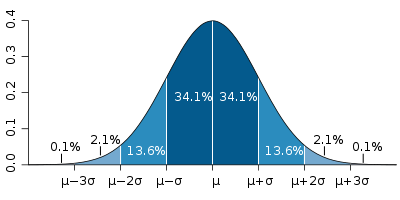
\includegraphics[width=0.8\linewidth]{./img/normal_distribution.png}

\begin{itemize}
    \item 68,27\% aller Werte im Intervall von einer Standardabweichung,
    \item 95,45\% aller Werte im Intervall von zwei Standardabweichungen
    \item 99,73\% aller Werte im Intervall von drei Standardabweichungen
\end{itemize}

\subsection{Seaborns jointplot}

\begin{minipage}{0.5\linewidth}
Der Jointplot ist eine verbindung von zwei Variablen mit bivariaten und univariaten Graphen. Es zeigt die (empirischen) Randverteilungen als Histogramme. Das Ergebnis ist ideal: die Daten (x-Werte) sind gleichmäßig über den gesamten Bereich verteilt (Gleichverteilung in -50/+50), während die Residuen bei 0 zentriert sind (Standardnormalverteilung).
\begin{minted}{python}
    penguins = sns.load_dataset("penguins")
    sns.jointplot(data=penguins, x="bill_length_mm", y="bill_depth_mm")
\end{minted}
\end{minipage}
\begin{minipage}{0.5\linewidth}
    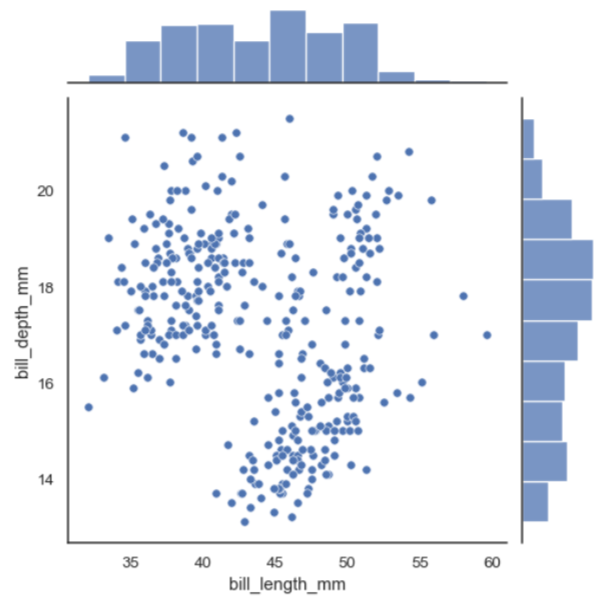
\includegraphics[width=\linewidth]{./img/sns_jointplot.png}
\end{minipage}


\subsection{Pearson Correlation Coefficient}
refers to the degree to which a pair of variables are linearly related. $0\rightarrow$ Kein Zusammenhang / $>0\rightarrow$ positiver Zusammenhang / $<0\rightarrow$ negativer (gegenläufiger) Zusammenhang.\\
\textbf{Achtung}: Beinhaltet keine Aussage über die Kausalität!  

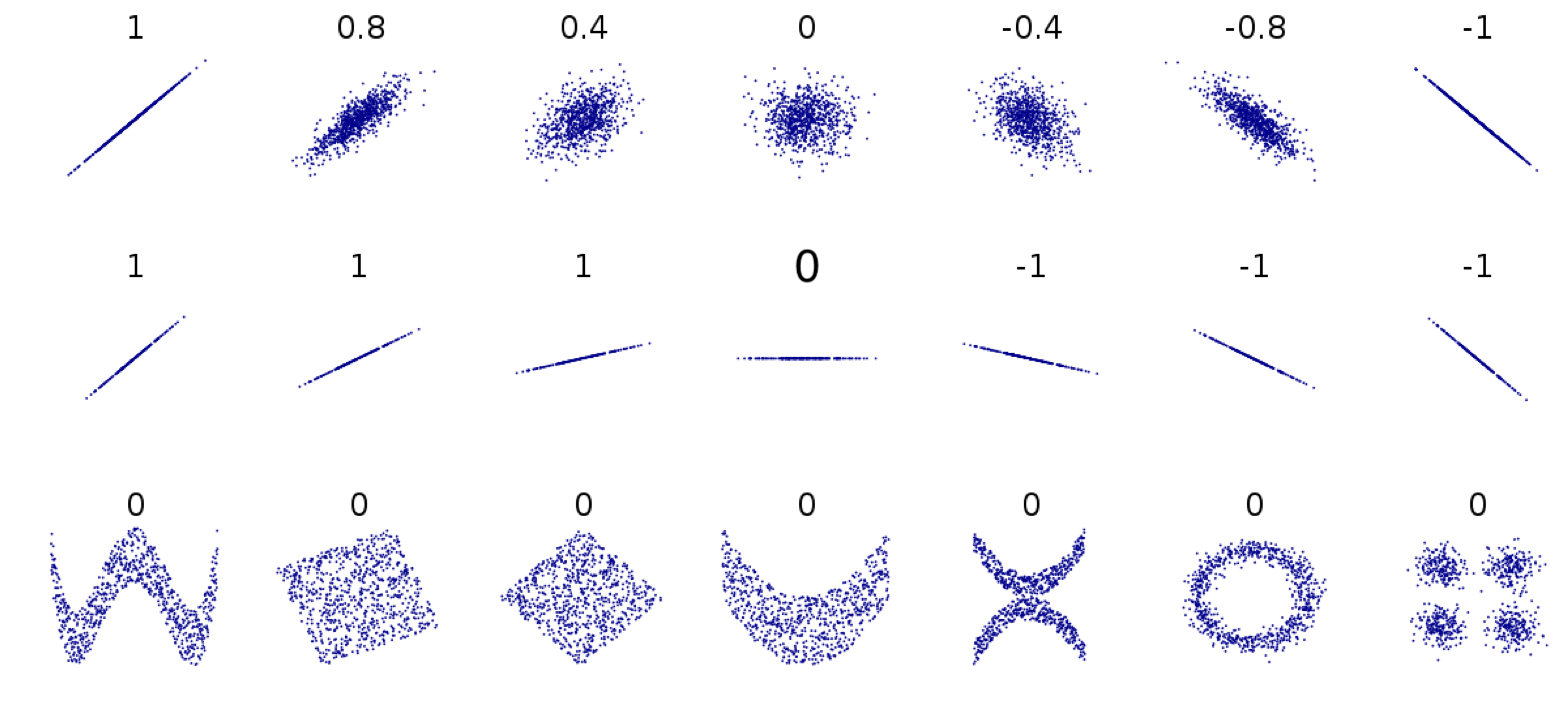
\includegraphics[width=\linewidth]{./img/pearson_correlation_coefficient.png}